\begin{figure}[htp]
	\centering
	\subfloat[\(\mesh{\Phi}\)]
	{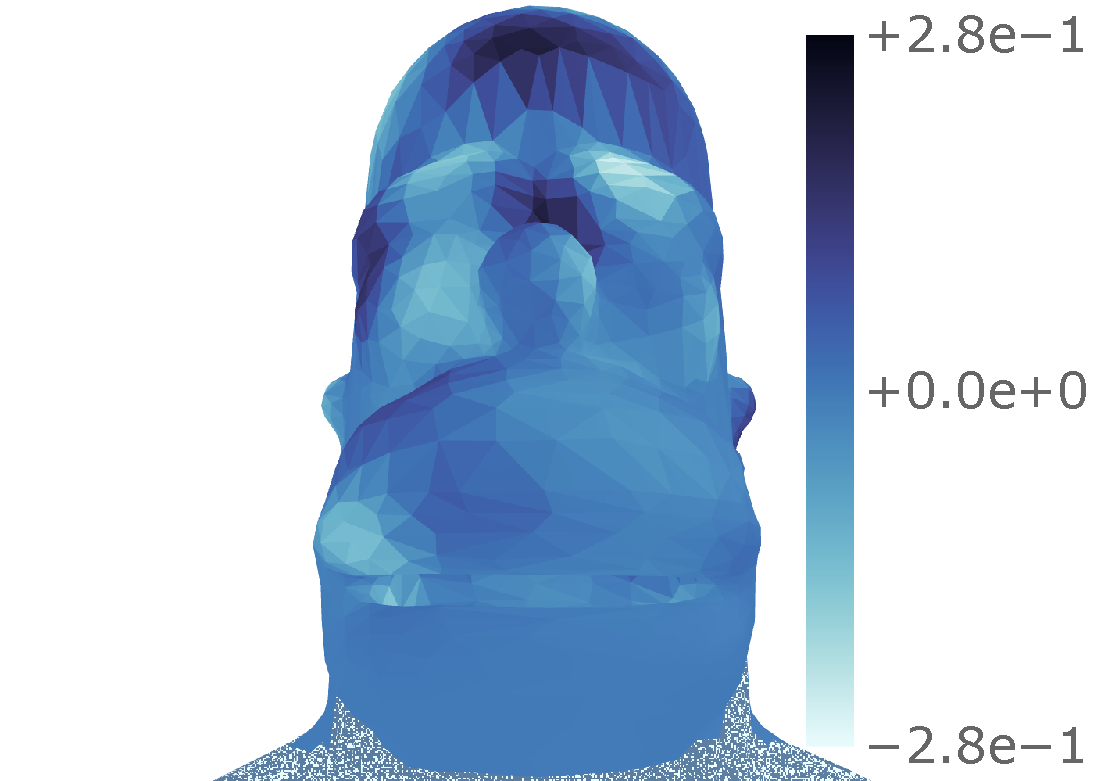
\includegraphics[trim={101 0 3 3},clip,width=.33\textwidth]{slepian_wavelets_homer_3B_2jmin_scaling_zoom.pdf}}
	\hfill
	\subfloat[\(\mesh{\Psi^{2j}}\)]
	{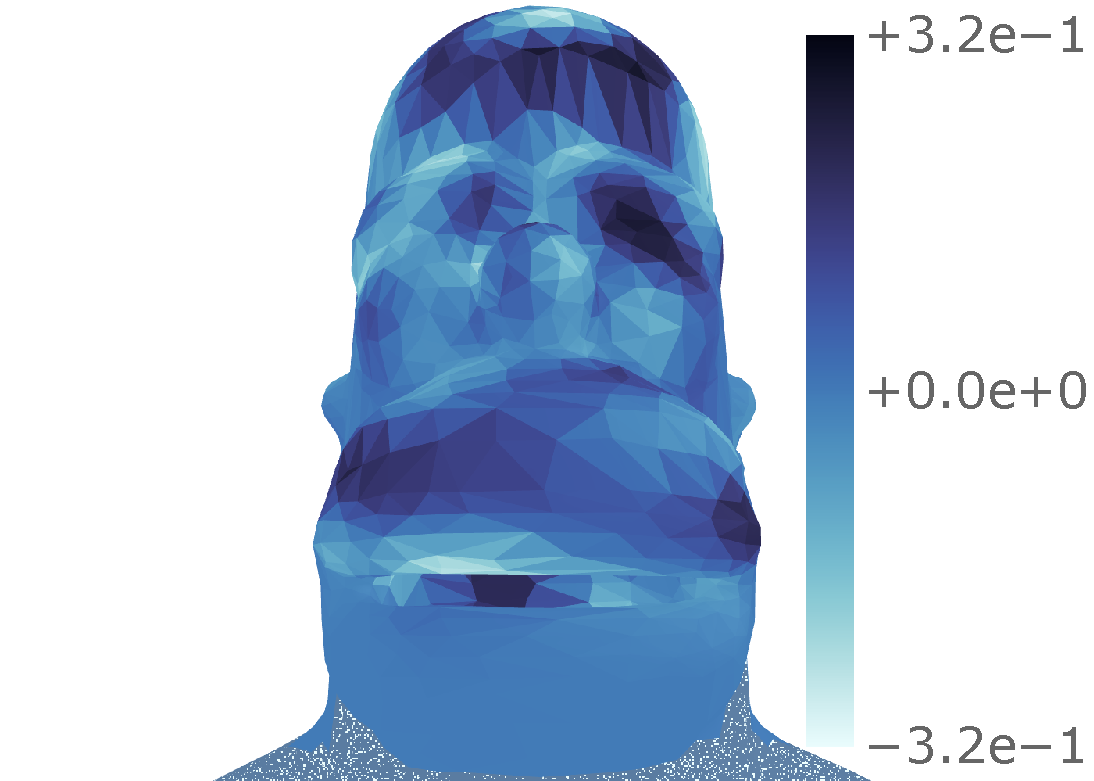
\includegraphics[trim={101 0 3 3},clip,width=.33\textwidth]{slepian_wavelets_homer_3B_2jmin_2j_zoom.pdf}}
	\hfill
	\subfloat[\(\mesh{\Psi^{3j}}\)]
	{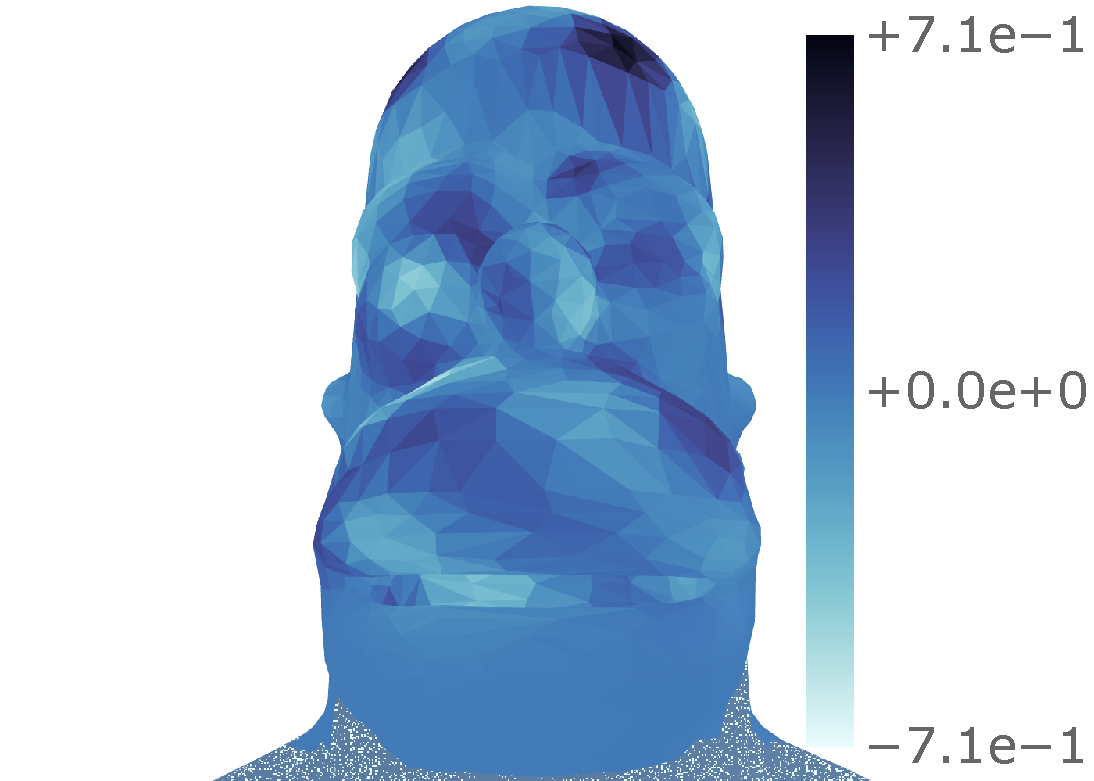
\includegraphics[trim={101 0 3 3},clip,width=.33\textwidth]{slepian_wavelets_homer_3B_2jmin_3j_zoom.pdf}}
	\newline
	\subfloat[\(\mesh{\Psi^{4j}}\)]
	{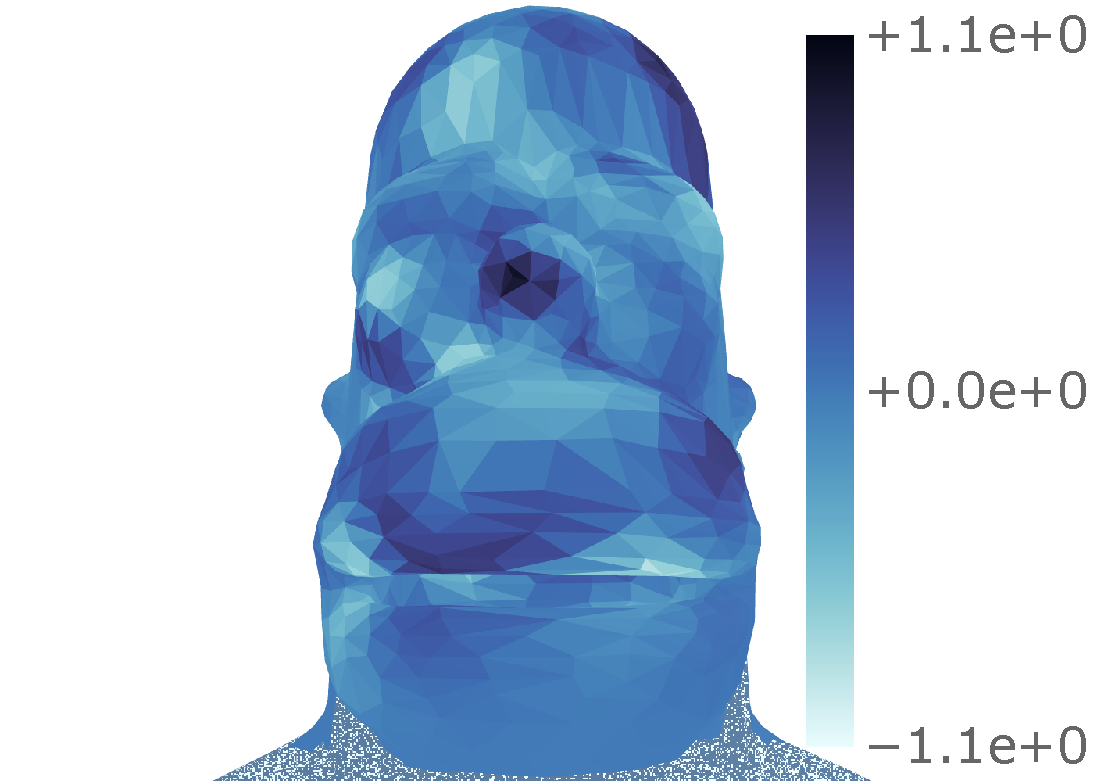
\includegraphics[trim={101 0 3 3},clip,width=.33\textwidth]{slepian_wavelets_homer_3B_2jmin_4j_zoom.pdf}}
	\hfill
	\subfloat[\(\mesh{\Psi^{5j}}\)]
	{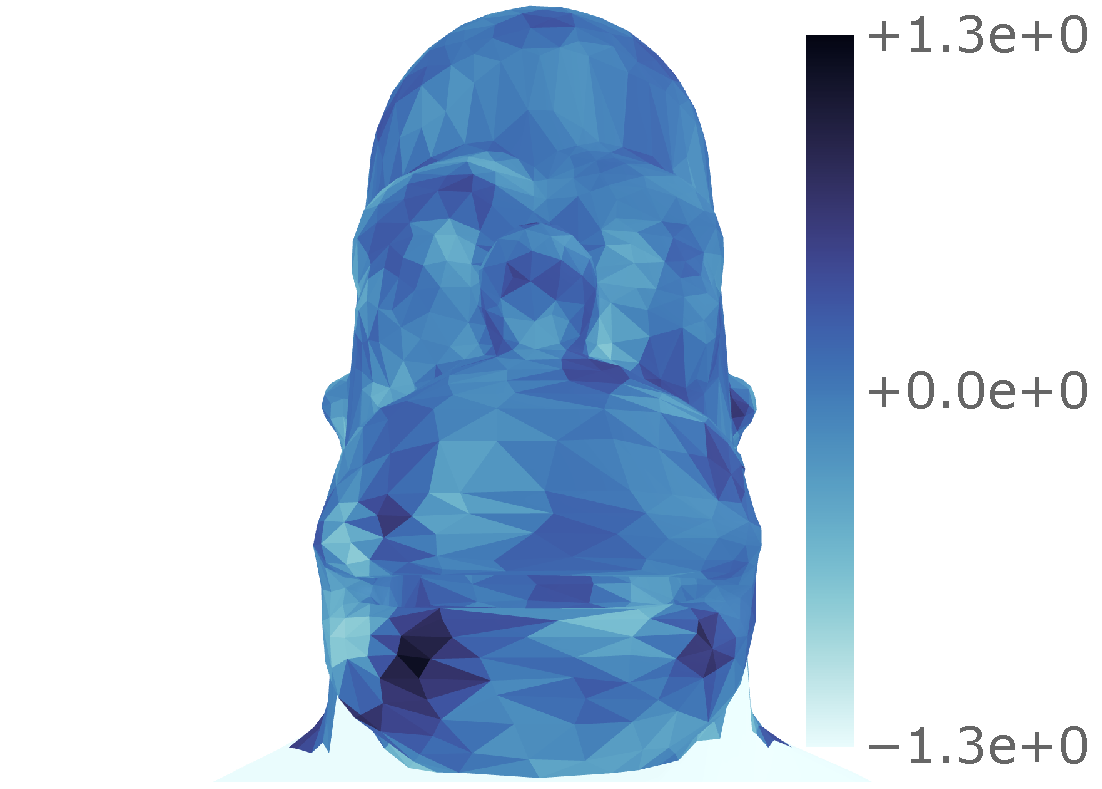
\includegraphics[trim={101 0 3 3},clip,width=.33\textwidth]{slepian_wavelets_homer_3B_2jmin_5j_zoom.pdf}}
	\hfill
	\subfloat[\(\mesh{\Psi^{6j}}\)]
	{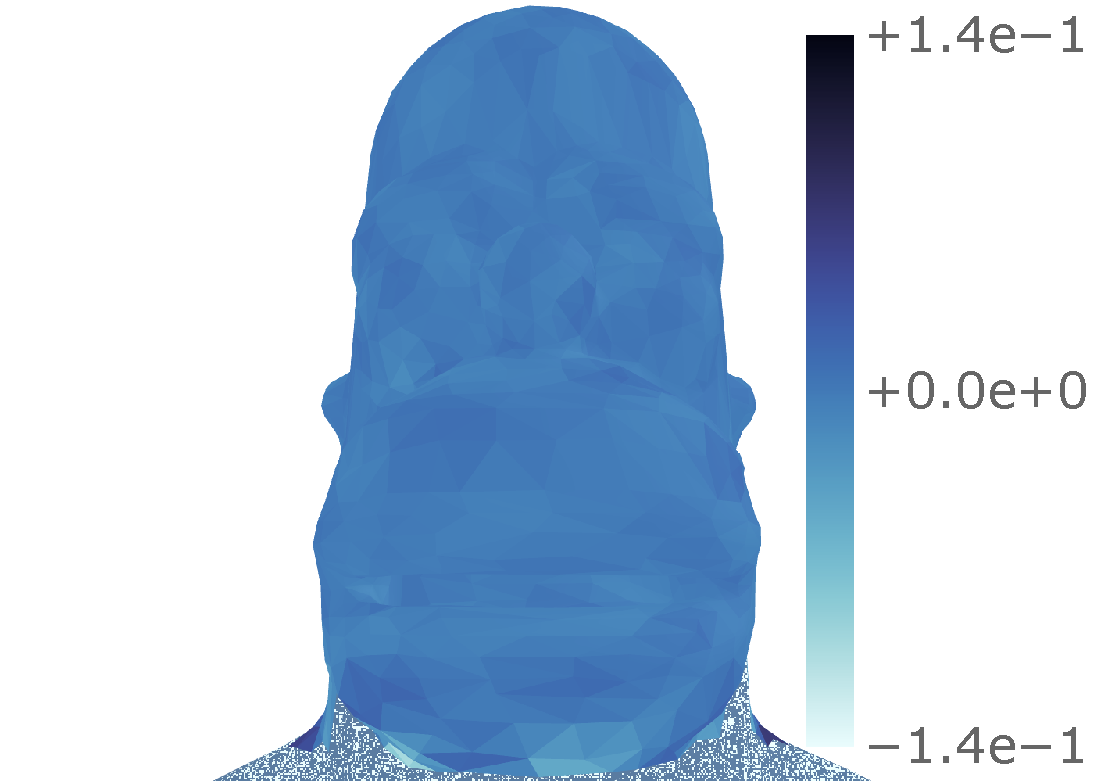
\includegraphics[trim={101 0 3 3},clip,width=.33\textwidth]{slepian_wavelets_homer_3B_2jmin_6j_zoom.pdf}}
	\caption{
		The scaling function and the wavelets for scales \(j \in \set{2, 3, 4, 5, 6}\) for the Homer head region shown left-to-right, top-to-bottom.
		The wavelets are constructed through a tiling of the Slepian line using scale-discretised functions, with parameters \(\lambda=3\), \(J_{0}=2\), and \(\num{1275}\) basis functions.
		Whilst the wavelets are defined on the vertices, the values have been averaged onto the faces for the plot.
	}\label{fig:chapter4_wavelets}
\end{figure}
